\documentclass[compress]{beamer}

\usepackage{tikz}
\usetikzlibrary{positioning, fit, calc, arrows.meta}

% \setbeamertemplate{footline}{eeee \insertframenumber}

% tikz config
\tikzset{block/.style={draw, thick, text width=1.8cm ,minimum height=1cm, align=center},
    line/.style={-latex}
}

\usetheme{CambridgeUS}
\usecolortheme{beaver}
\useoutertheme[subsection=false]{miniframes}
\setbeamertemplate{caption}[numbered]


\title[558 Project: Packet Scheduling]{Analysis of Packet Scheduling using Network Simulation}
\author[Ethan Ruchotzke]{Ethan Ruchotzke}
\institute[]{CprE 558\\Iowa State University}
\date{\today}

\begin{document}

    \frame{\titlepage}


    \section{Problem Statement}

    \subsection{Problem Statement}
    \begin{frame}
        \frametitle{Problem Statement}
        \begin{itemize}
            \item Modern internetworking is built for "best effort" scheduling
            \item Real time networks demand packet scheduling with different properties
            \begin{itemize}
                \item Fairness (typical, max-min)
            \end{itemize}
            \item Demand to investigate packet schedulers and identify their impact on flows
        \end{itemize}
    \end{frame}


    \section{Solution}

    \subsection{1}
    \begin{frame}
        \frametitle{Solution}
        \begin{itemize}
            \item Simulation!
            \item Work through theoretical flows of packets
            \begin{itemize}
                \item Fast, easy to implement many test cases
                \item Easy to implement routing schemes
            \end{itemize}
            \item Easy to pull results from simulated network without noise/interference
        \end{itemize}
    \end{frame}


    \section{Implementation Details}

    \subsection{Choices}
    \begin{frame}
        \frametitle{Network Simulation Choices}
        \begin{columns}
            \begin{column}{0.5\textwidth}
                \begin{itemize}
                    \item Many options
                    \begin{itemize}
                        \item NS-3 \alert{(hard to tweak for experiments on scheduling)}
                        \item Mininet \alert{(focused on SDNs/higher-level changes)}
                        \item GNS-3 \alert{(too intensive/large)}
                    \end{itemize}
                    \item I decided to roll my own, since I had the experience to do so
                    \begin{itemize}
                        \item SimPy - Discrete Event Simulator
                    \end{itemize}
                \end{itemize}
            \end{column}
            \begin{column}{0.5\textwidth}
                \begin{figure}
                    \centering
                    
\includegraphics[width=0.5\textwidth]{img/ns-3.png}
                \end{figure}
                \begin{figure}
                    \centering
                    
\includegraphics[width=0.3\textwidth]{img/GNS3_logo.png}
                \end{figure}
                \begin{figure}
                    \centering
                    
\includegraphics[width=0.5\textwidth]{img/SimPy.png}
                \end{figure}
            \end{column}
        \end{columns}
    \end{frame}

    \subsection{Implementation}
    \begin{frame}
        \frametitle{Network Simulation}
        \begin{columns}
            \begin{column}{0.7\textwidth}
                \begin{itemize}
                    \item Two major components
                    \begin{itemize}
                        \item Nodes (contain a network stack)
                        \item Networks (equivalent to CSMA network)
                    \end{itemize}
                    \item Networks have a bandwidth which limits transmission time
                    \item Nodes must wait for the shared resource (network) before transmitting
                    \item Nodes run applications and various network layers
                \end{itemize}
            \end{column}

            \begin{column}{0.3\textwidth}
                \begin{figure}
                    \centering
                    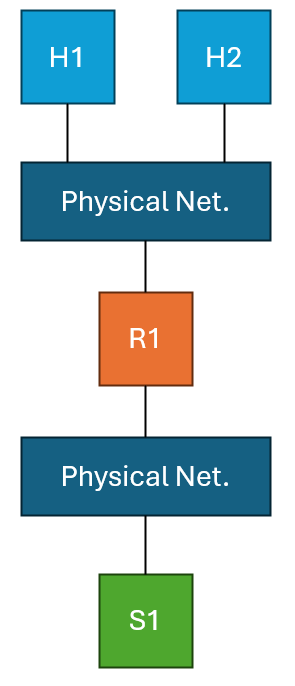
\includegraphics[width=0.8\textwidth]{img/example-net}
                \end{figure}
            \end{column}
        \end{columns}
    \end{frame}

    \subsection{2}
    \begin{frame}
        \frametitle{Network Stack}
        \begin{columns}
            \begin{column}{0.5\textwidth}
                \begin{itemize}
                    \item Replicate the layers of an actual network
                    \begin{itemize}
                        \item Ethernet: Physical network access, filtering
                        \item IP: Routing
                        \item App: Generation/consumption
                    \end{itemize}
                    \item Multiple layers of a type allowed (routers have two interfaces)
                    \item IP Layer handles packet queueing (of interest to project)
                    \item Everything implemented to account for queueing delays/latency
                \end{itemize}
            \end{column}

            \begin{column}{0.5\textwidth}
                \begin{figure}
                    \centering
                    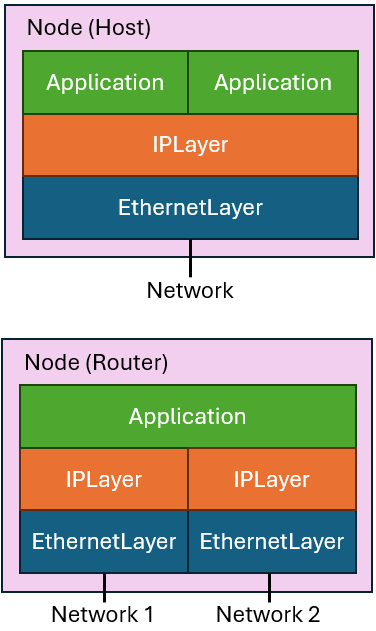
\includegraphics[width=0.6\textwidth]{img/combo}
                \end{figure}
            \end{column}
        \end{columns}
    \end{frame}

    \subsection{3}
    \begin{frame}
        \frametitle{Discipline}
        \begin{columns}
            \begin{column}{0.5\textwidth}
                \begin{itemize}
                    \item Handle prioritization/ordering of traffic
                    \item Traffic incoming from HW layer is queued by flow
                    \item Discipline pulls from flows and stores into output queue
                    \item Three disciplines of interest
                    \begin{itemize}
                        \item FIFO: Single input queue
                        \item Round Robin: Equally service multiple flows
                        \item Fair Queue: Fairly service multiple flows
                    \end{itemize}
                \end{itemize}
            \end{column}

            \begin{column}{0.5\textwidth}
                \begin{figure}
                    \centering
                    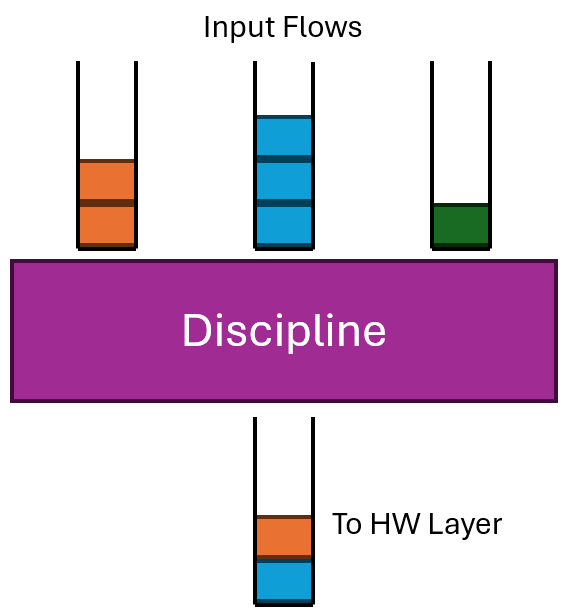
\includegraphics[width=0.7\textwidth]{img/discipline}
                \end{figure}
            \end{column}
        \end{columns}
    \end{frame}


    \section{Testing and Evaluation}

    \subsection{1}
    \begin{frame}
        \frametitle{Test Setup}

        \begin{itemize}
            \item Two networks
            \begin{itemize}
                \item Input network high bandwidth
                \item Output network variable (low, med, high)
            \end{itemize}
            \item Three flows
            \begin{itemize}
                \item Equivalent bandwidth (100 bs)
                \item Different levels of packets (5/s, 1/s, 0.5/s)
            \end{itemize}
            \item One router with tested discipline
        \end{itemize}

        \begin{figure}[b]
            \centering
            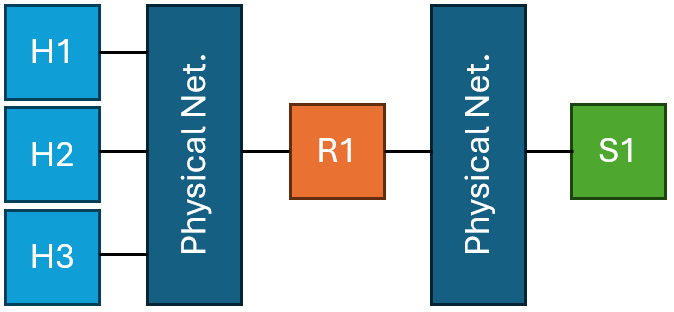
\includegraphics[height=0.2\textheight]{img/test-network}
        \end{figure}
    \end{frame}

    \subsection{2}
    \begin{frame}
        \frametitle{Results - Fairness}
        \begin{columns}
            \begin{column}{0.3\textwidth}
                \begin{tabular}{|c|c|c|}
                    \hline
                    Flow & P. Size & Period \\
                    \hline
                    1    & 100     & 1s     \\
                    2    & 20      & 0.2s   \\
                    3    & 200     & 2s     \\
                    \hline
                \end{tabular}
            \end{column}

            \begin{column}{0.7\textwidth}
                \begin{figure}
                    \centering
                    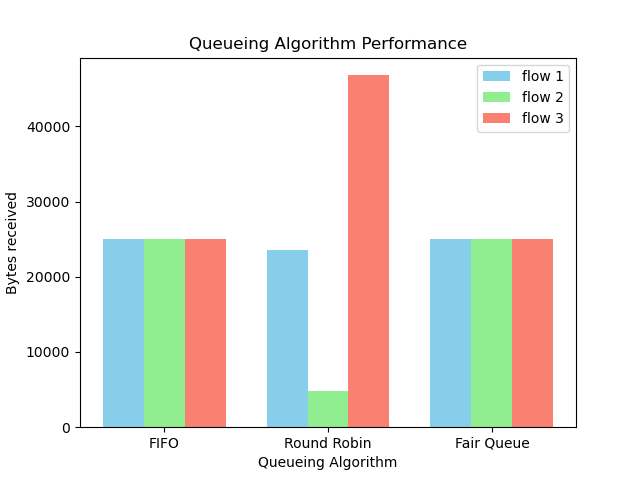
\includegraphics[width=0.9\textwidth]{img/fairness_bar}
                \end{figure}
            \end{column}
        \end{columns}
    \end{frame}

    \subsection{3}
    \begin{frame}
        \frametitle{Results - Latency (congested)}
        \begin{columns}
            \begin{column}{0.5\textwidth}
                \begin{figure}
                    \centering
                    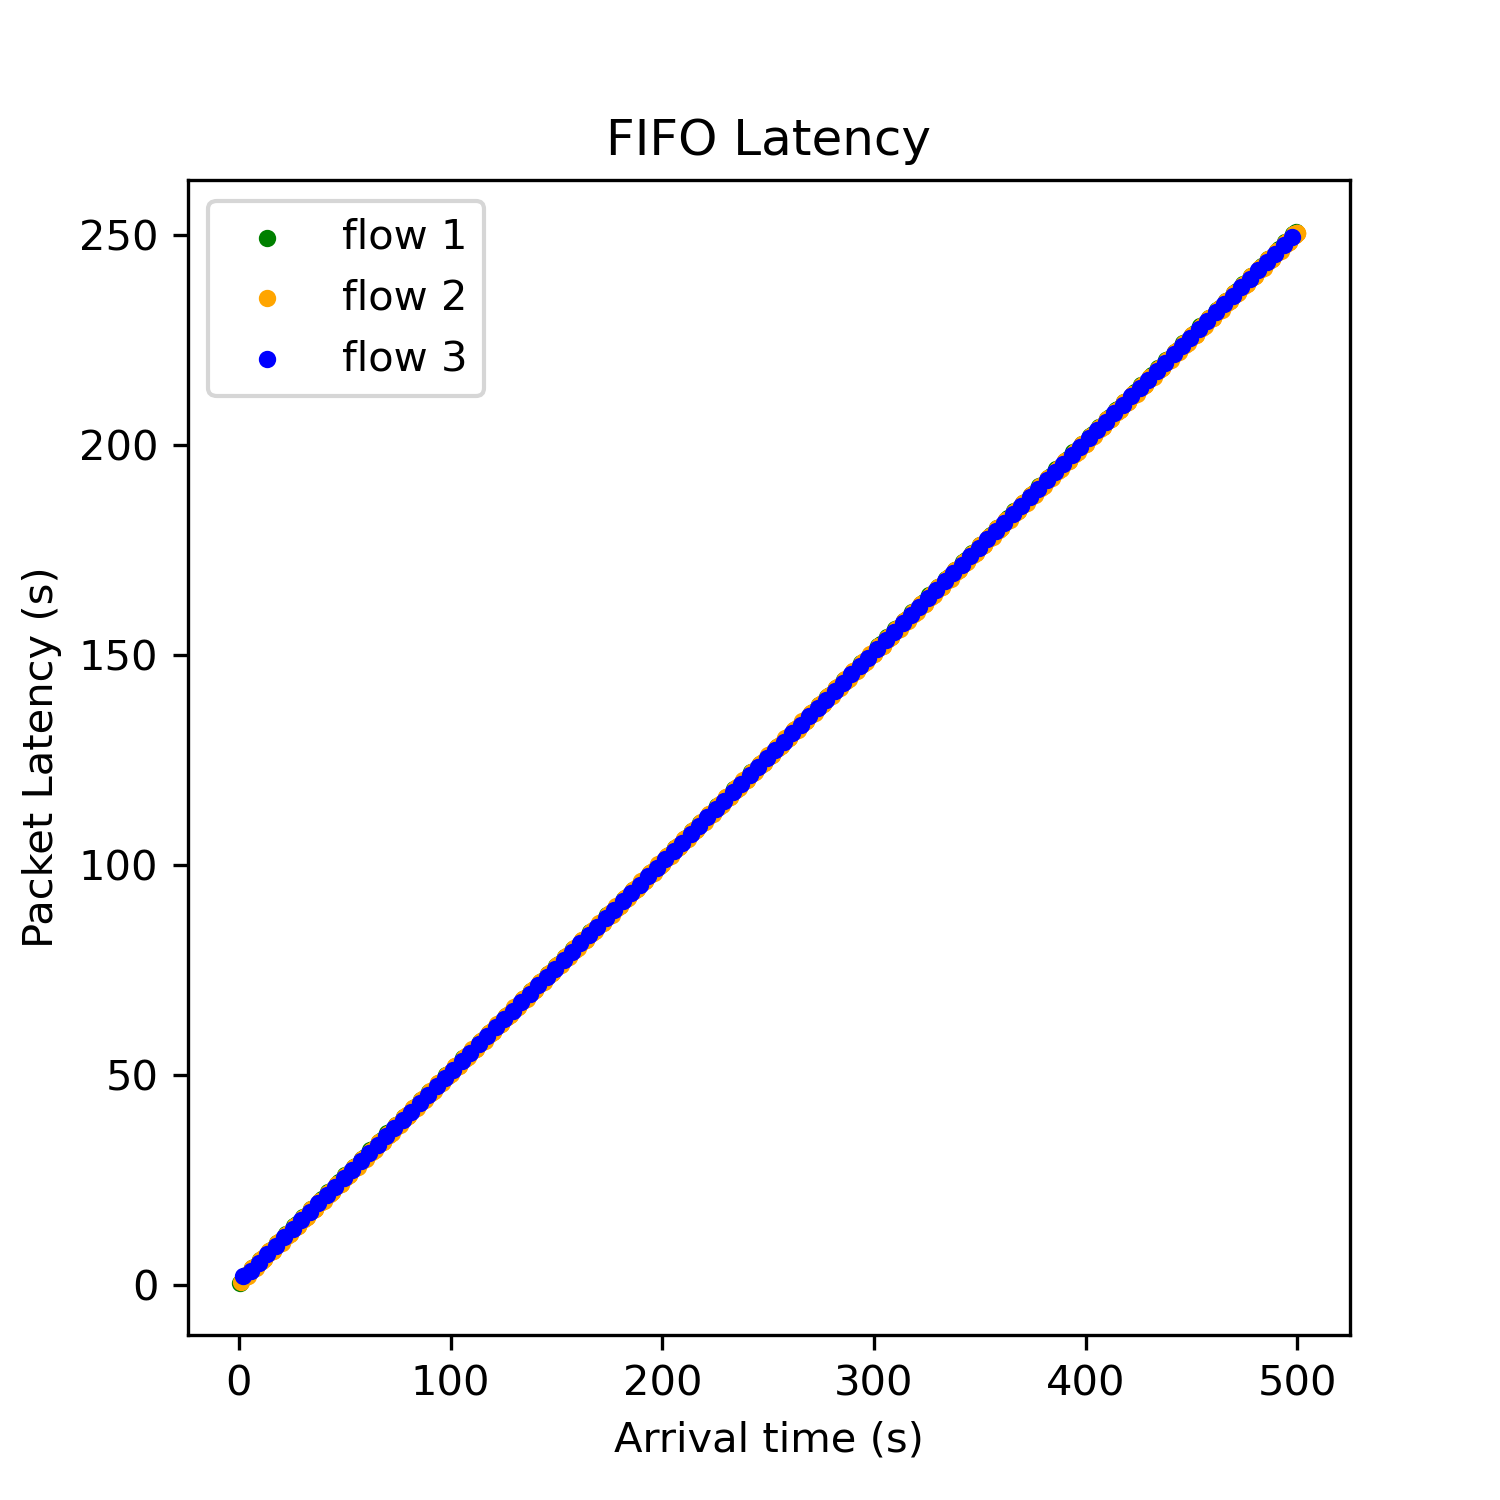
\includegraphics[width=\textwidth]{img/FIFO_Latency}
                \end{figure}
            \end{column}
            \begin{column}{0.5\textwidth}
                \begin{figure}
                    \centering
                    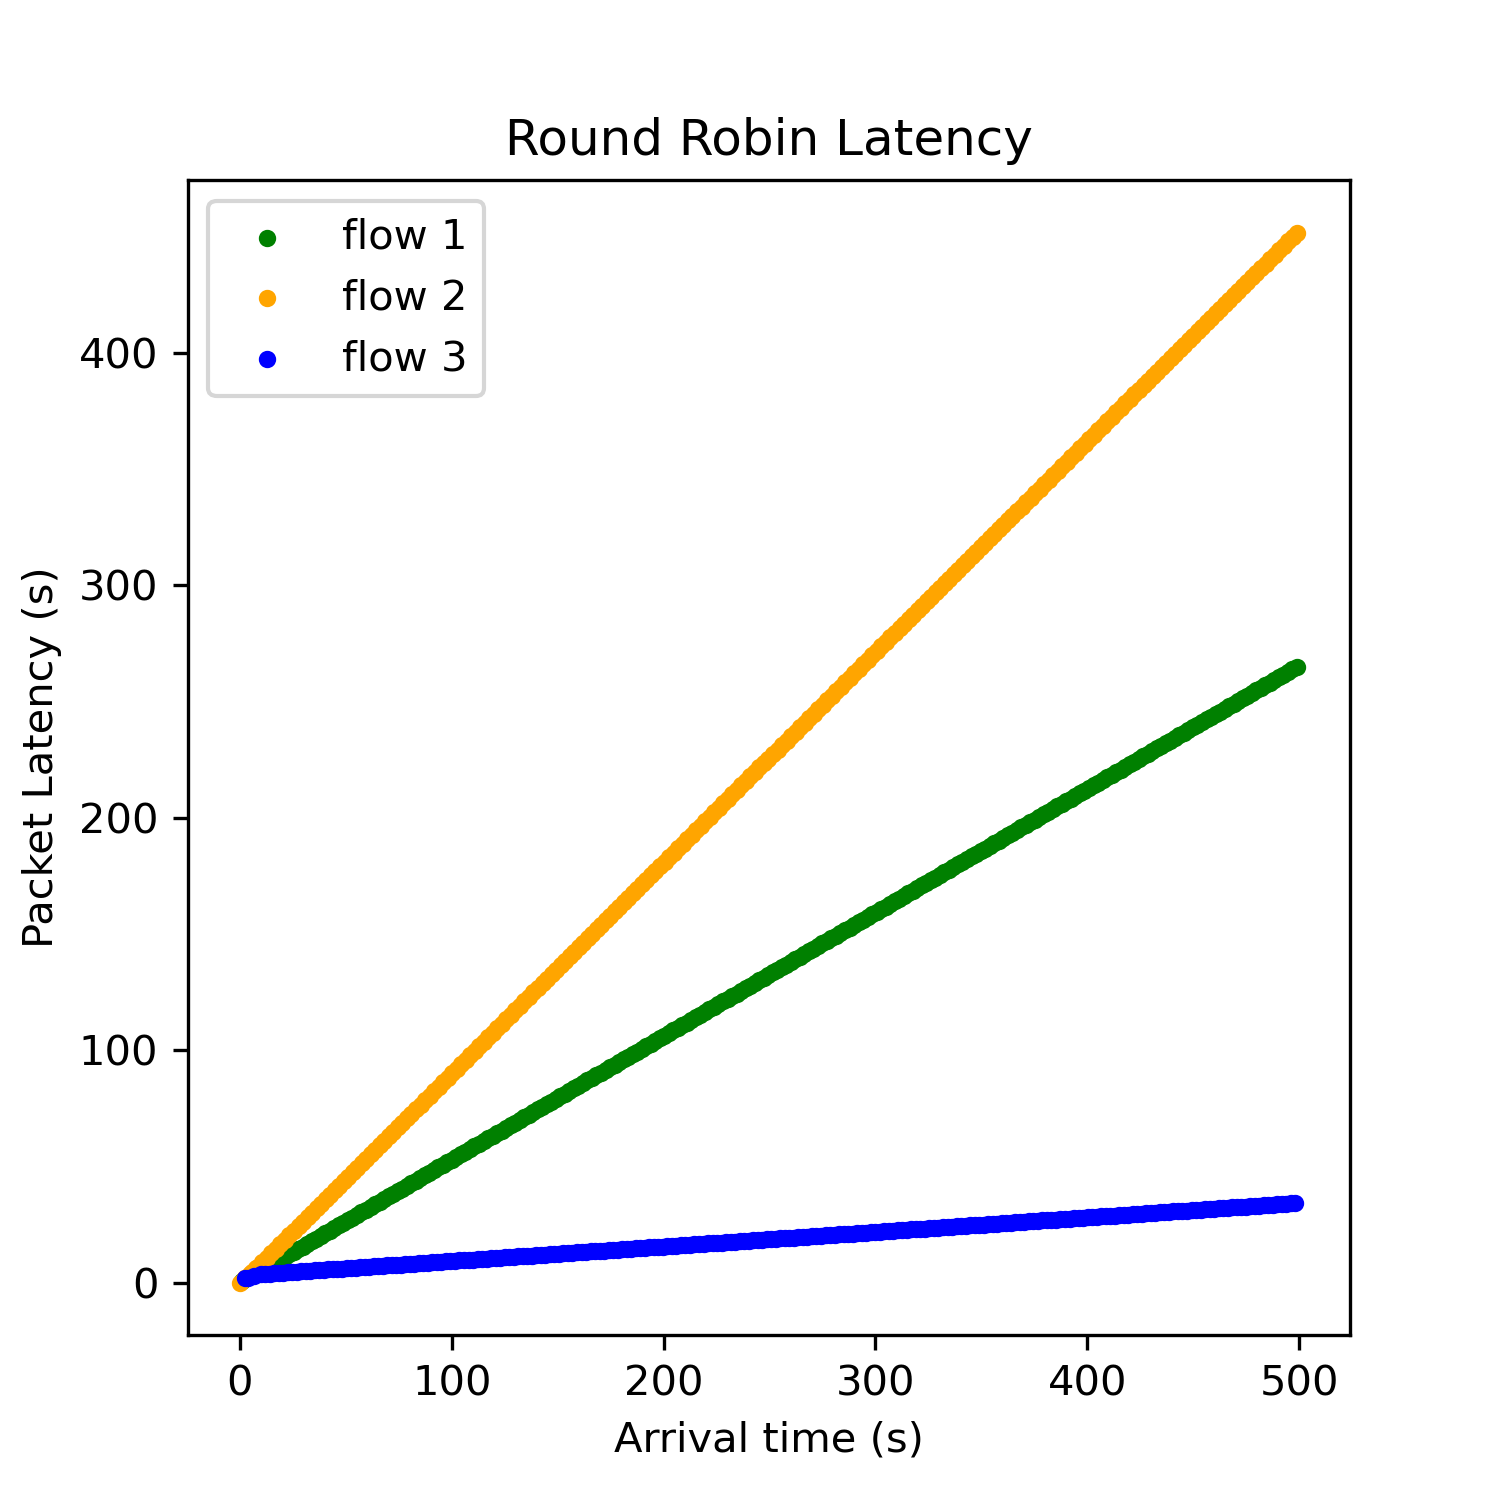
\includegraphics[width=\textwidth]{img/rr_latency}
                \end{figure}
            \end{column}
%            \begin{column}{0.3\textwidth}
%                \begin{figure}
%                    \centering
%                    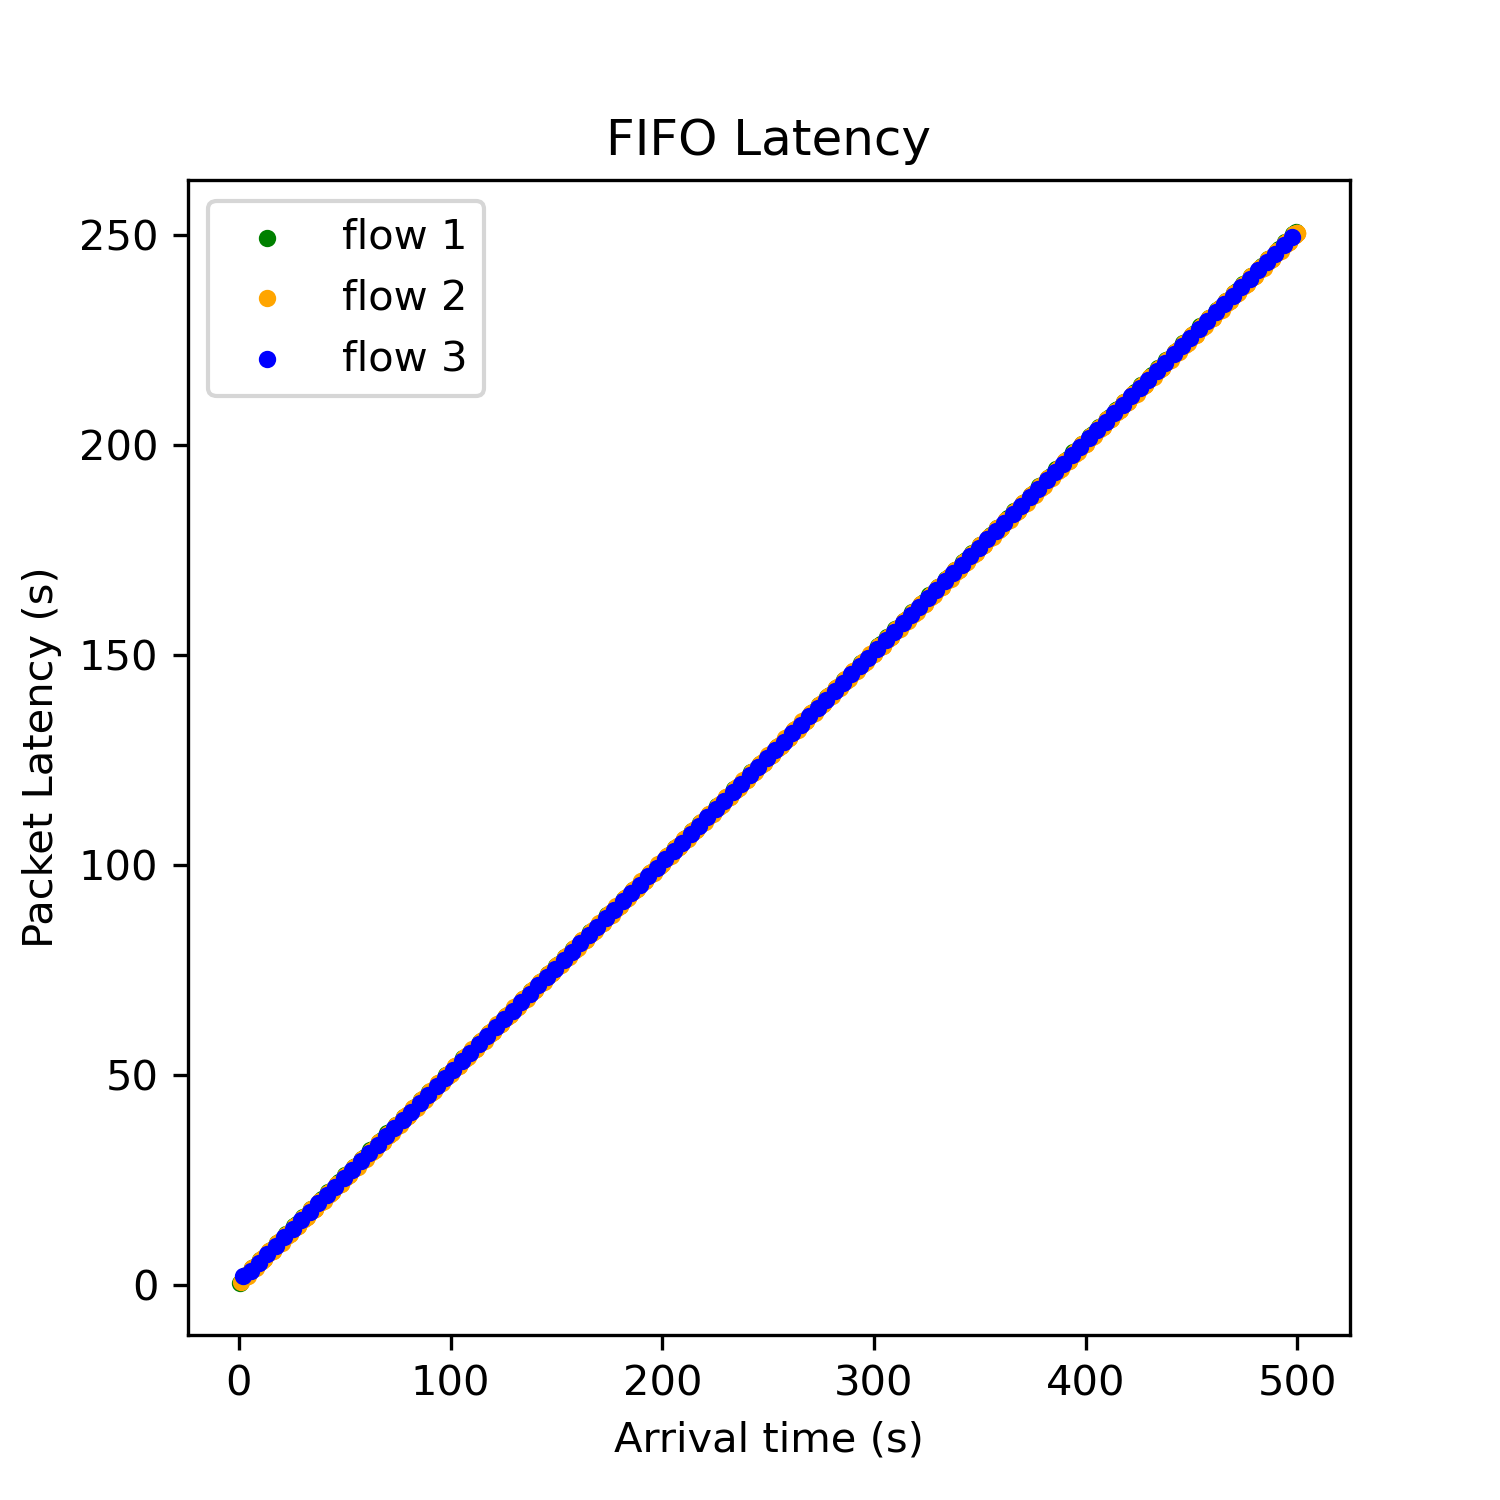
\includegraphics[width=\textwidth]{img/FIFO_Latency}
%                \end{figure}
%            \end{column}
        \end{columns}
    \end{frame}

    \subsection{4}
    \begin{frame}
        \frametitle{Results - Latency (equal)}
        \begin{columns}
            \begin{column}{0.32\textwidth}
                \begin{figure}
                    \centering
                    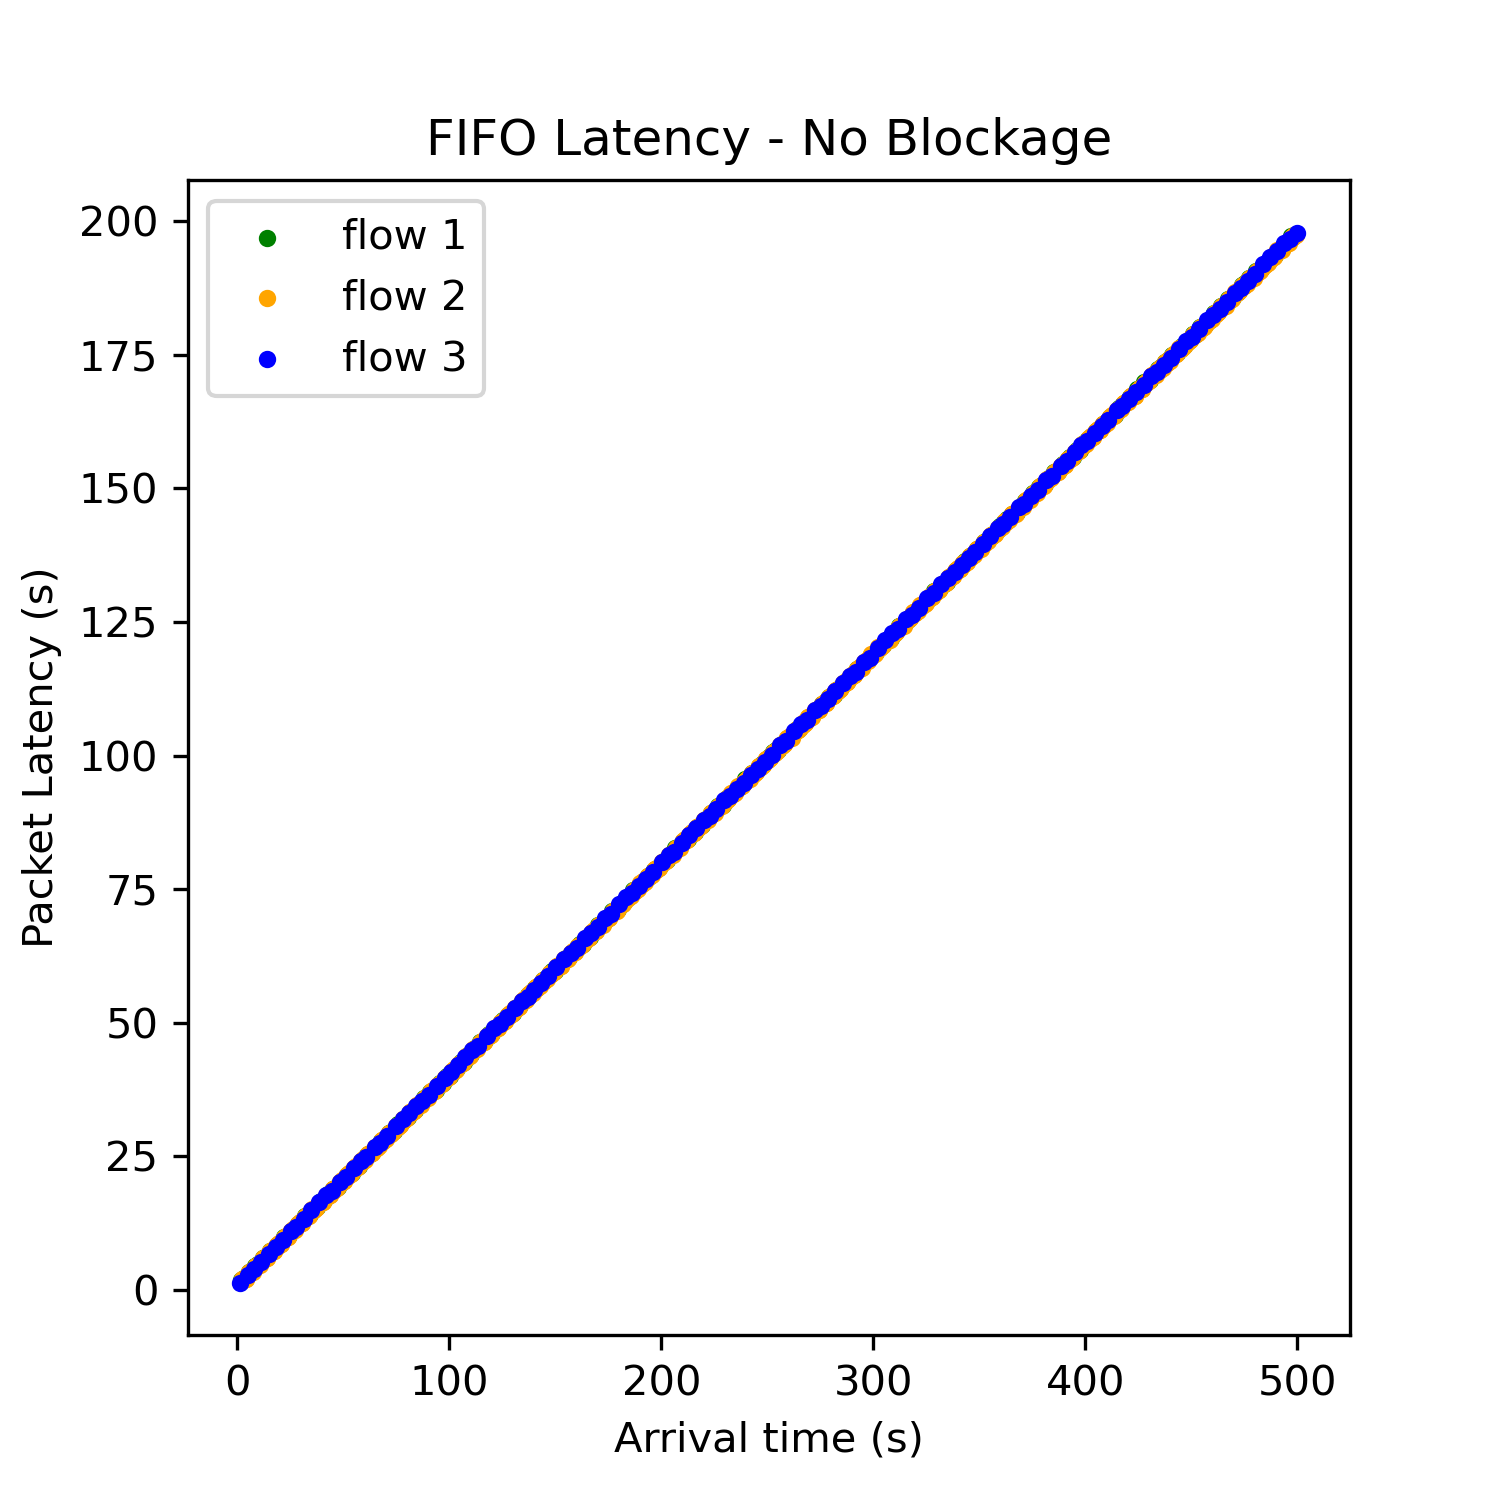
\includegraphics[width=\textwidth]{img/fifo_equal}
                \end{figure}
            \end{column}
            \begin{column}{0.32\textwidth}
                \begin{figure}
                    \centering
                    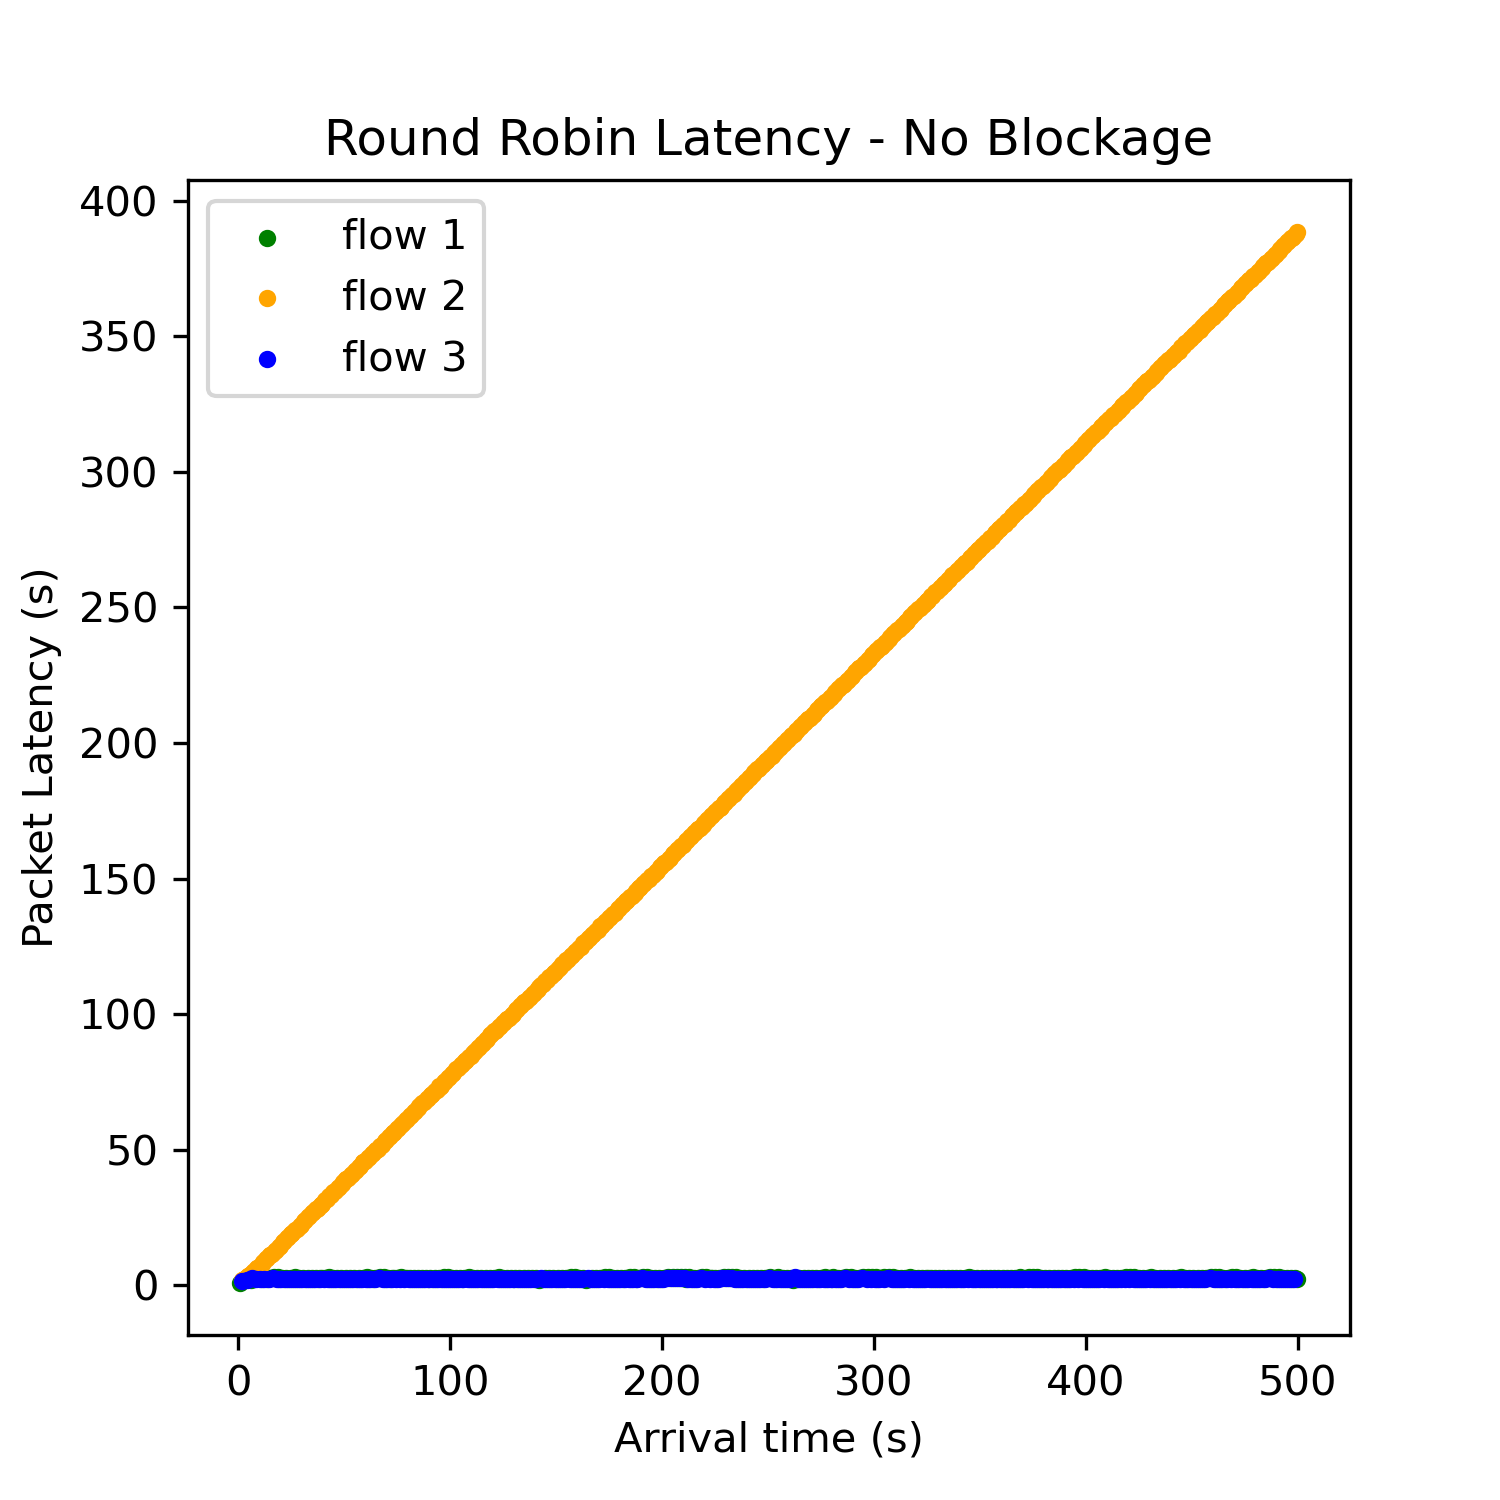
\includegraphics[width=\textwidth]{img/rr_equal}
                \end{figure}
            \end{column}
            \begin{column}{0.32\textwidth}
                \begin{figure}
                    \centering
                    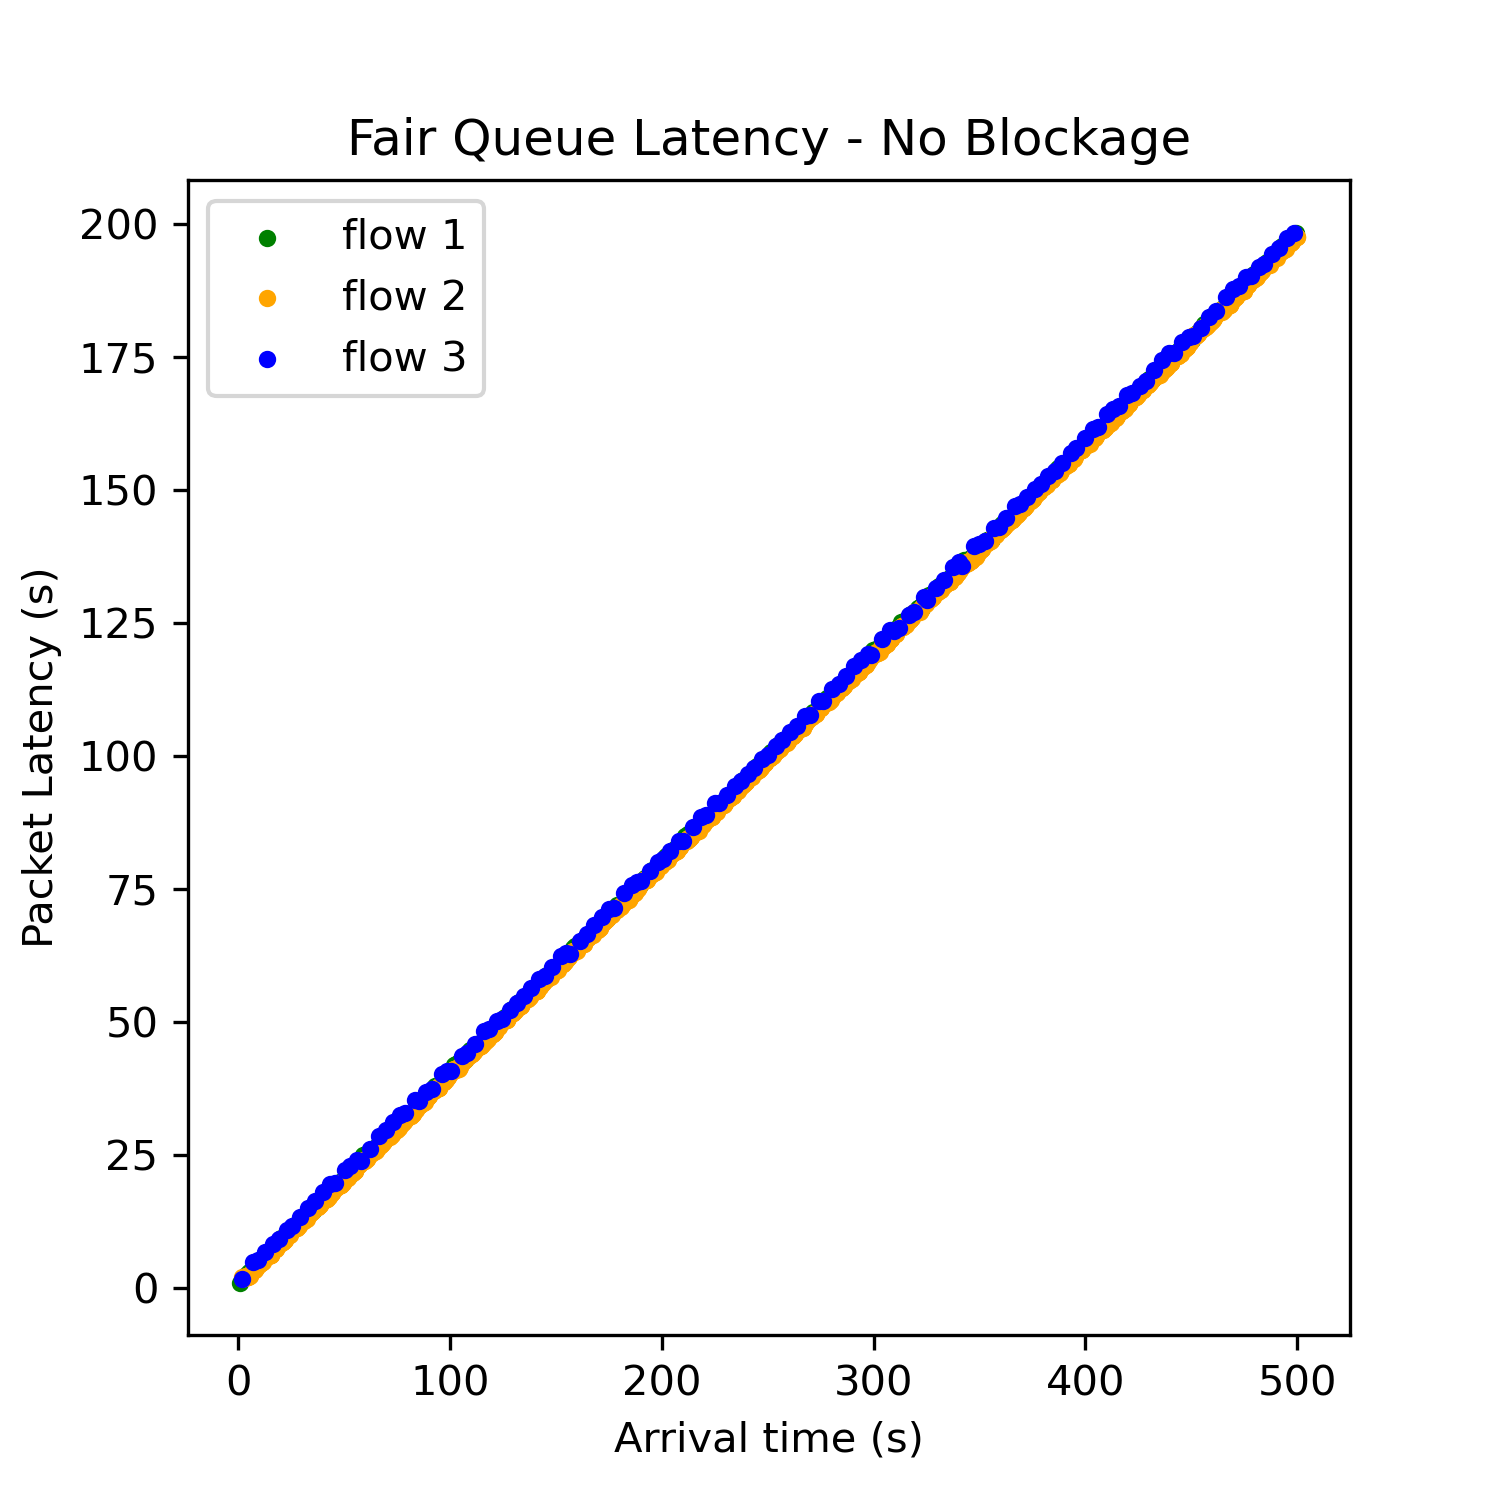
\includegraphics[width=\textwidth]{img/fq_equal}
                \end{figure}
            \end{column}
        \end{columns}
    \end{frame}

    \subsection{5}
    \begin{frame}
        \frametitle{Results - Latency (excess)}
        \begin{columns}
            \begin{column}{0.32\textwidth}
                \begin{figure}
                    \centering
                    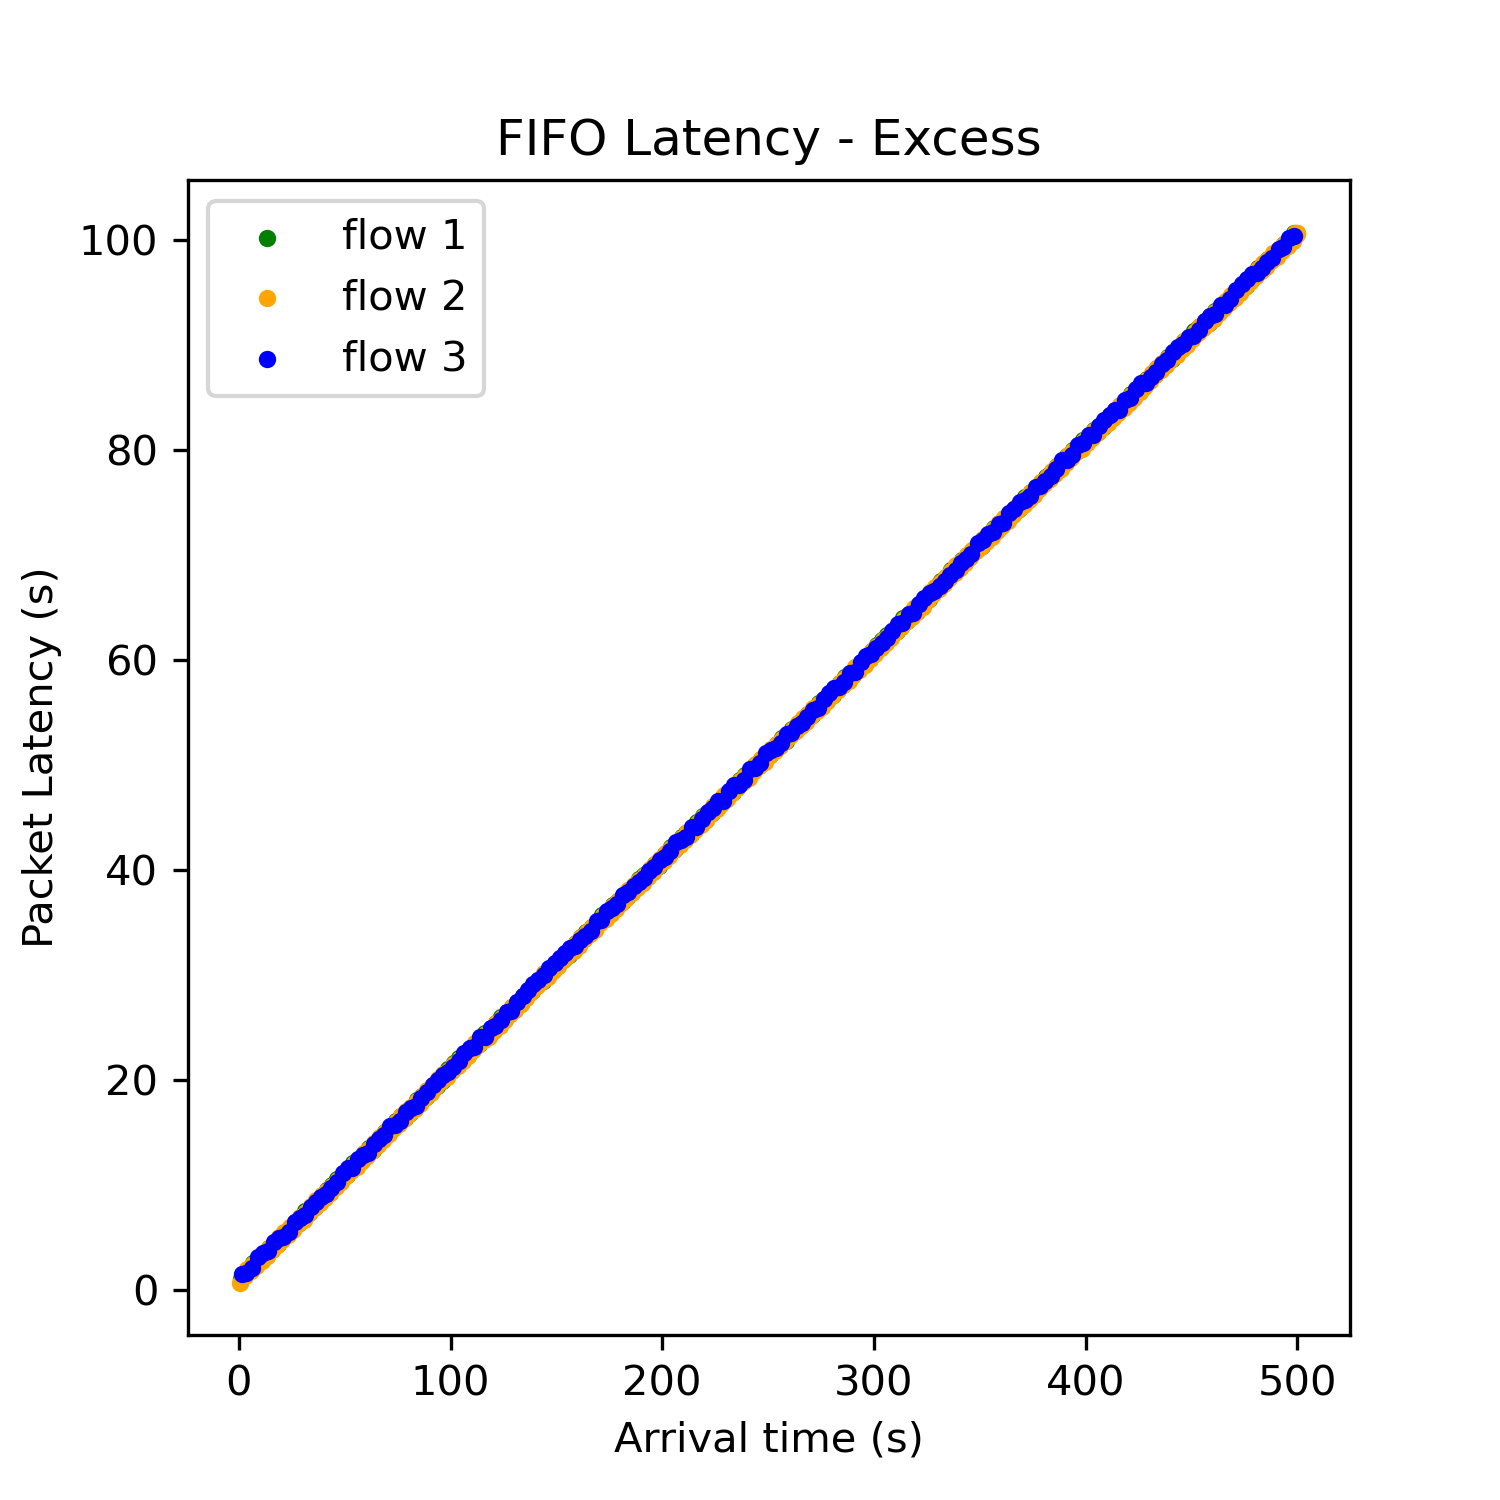
\includegraphics[width=\textwidth]{img/fifo_excess}
                \end{figure}
            \end{column}
            \begin{column}{0.32\textwidth}
                \begin{figure}
                    \centering
                    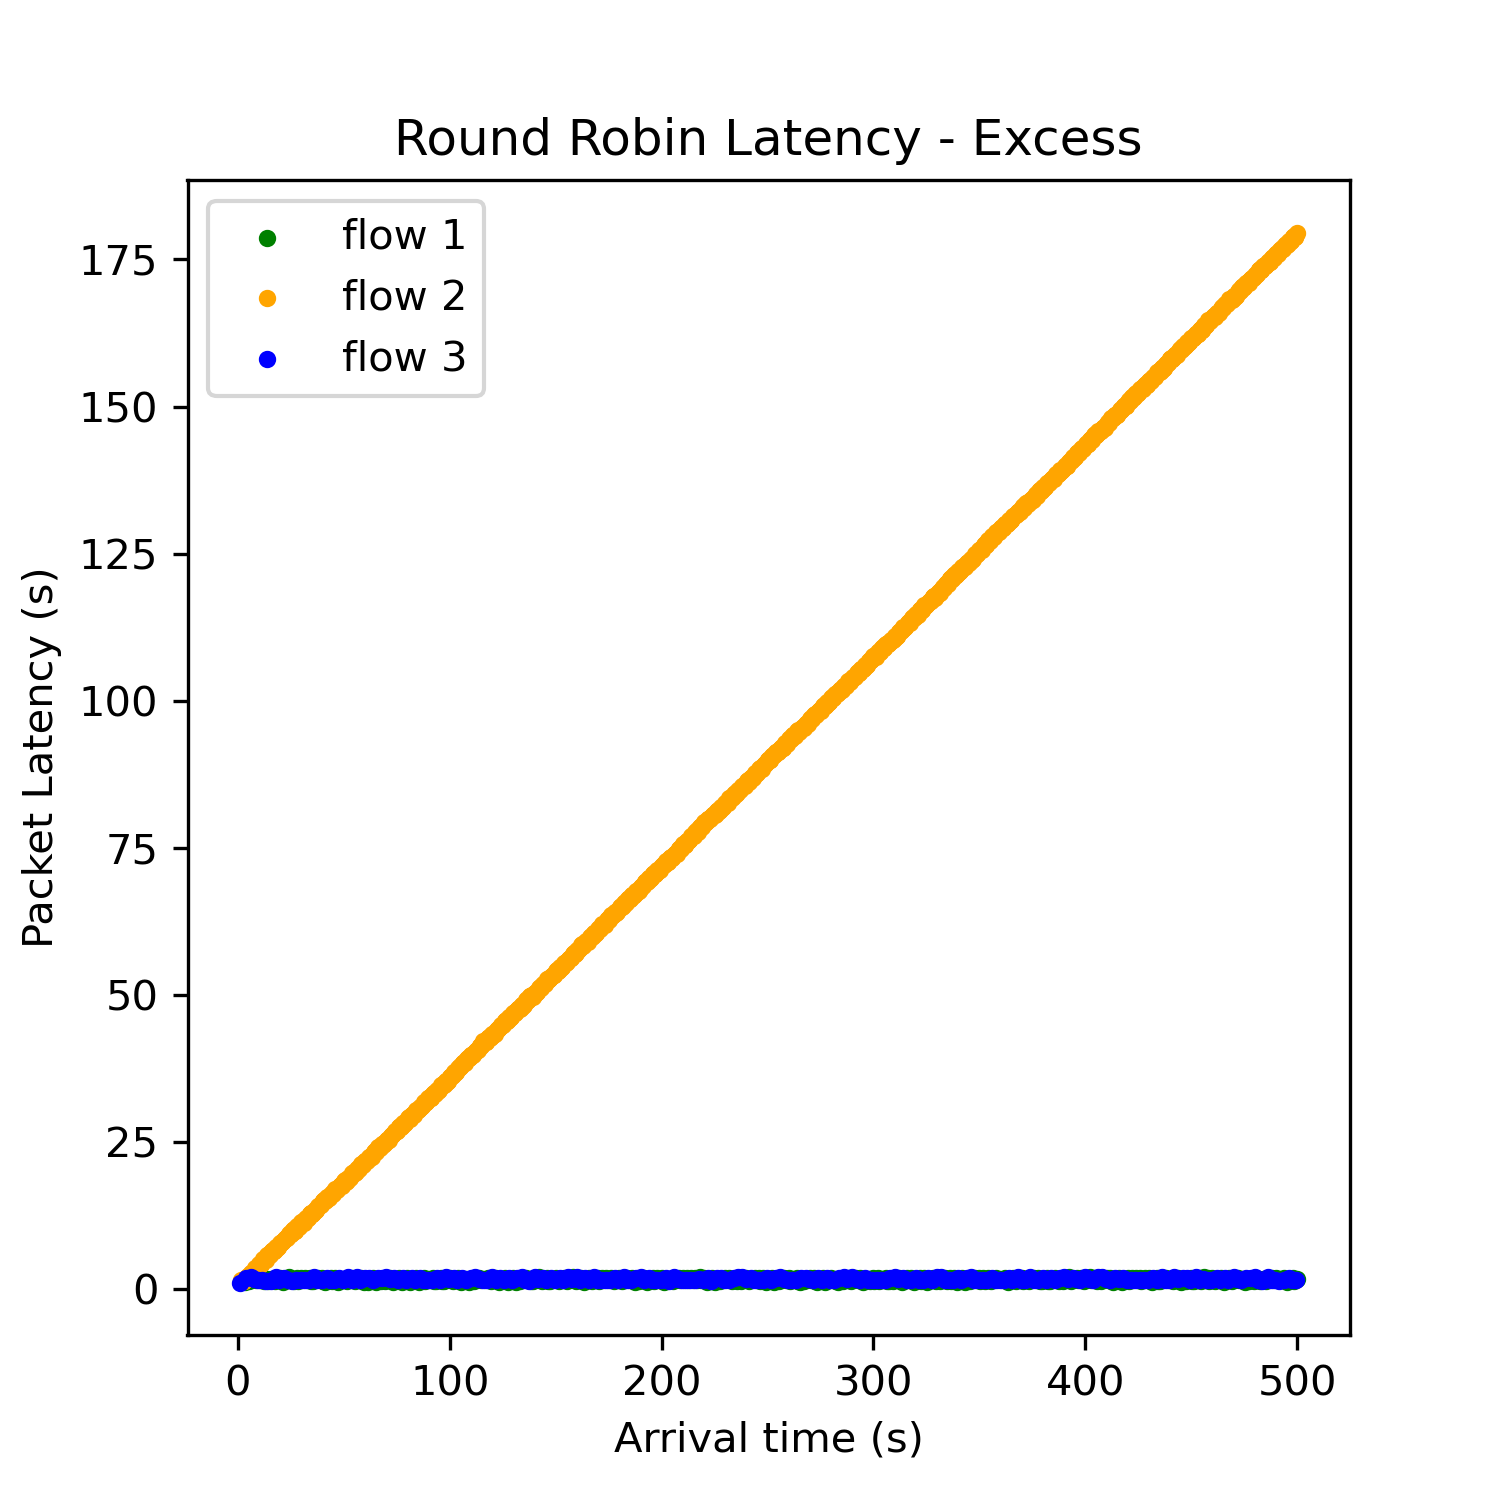
\includegraphics[width=\textwidth]{img/rr_excess}
                \end{figure}
            \end{column}
            \begin{column}{0.32\textwidth}
                \begin{figure}
                    \centering
                    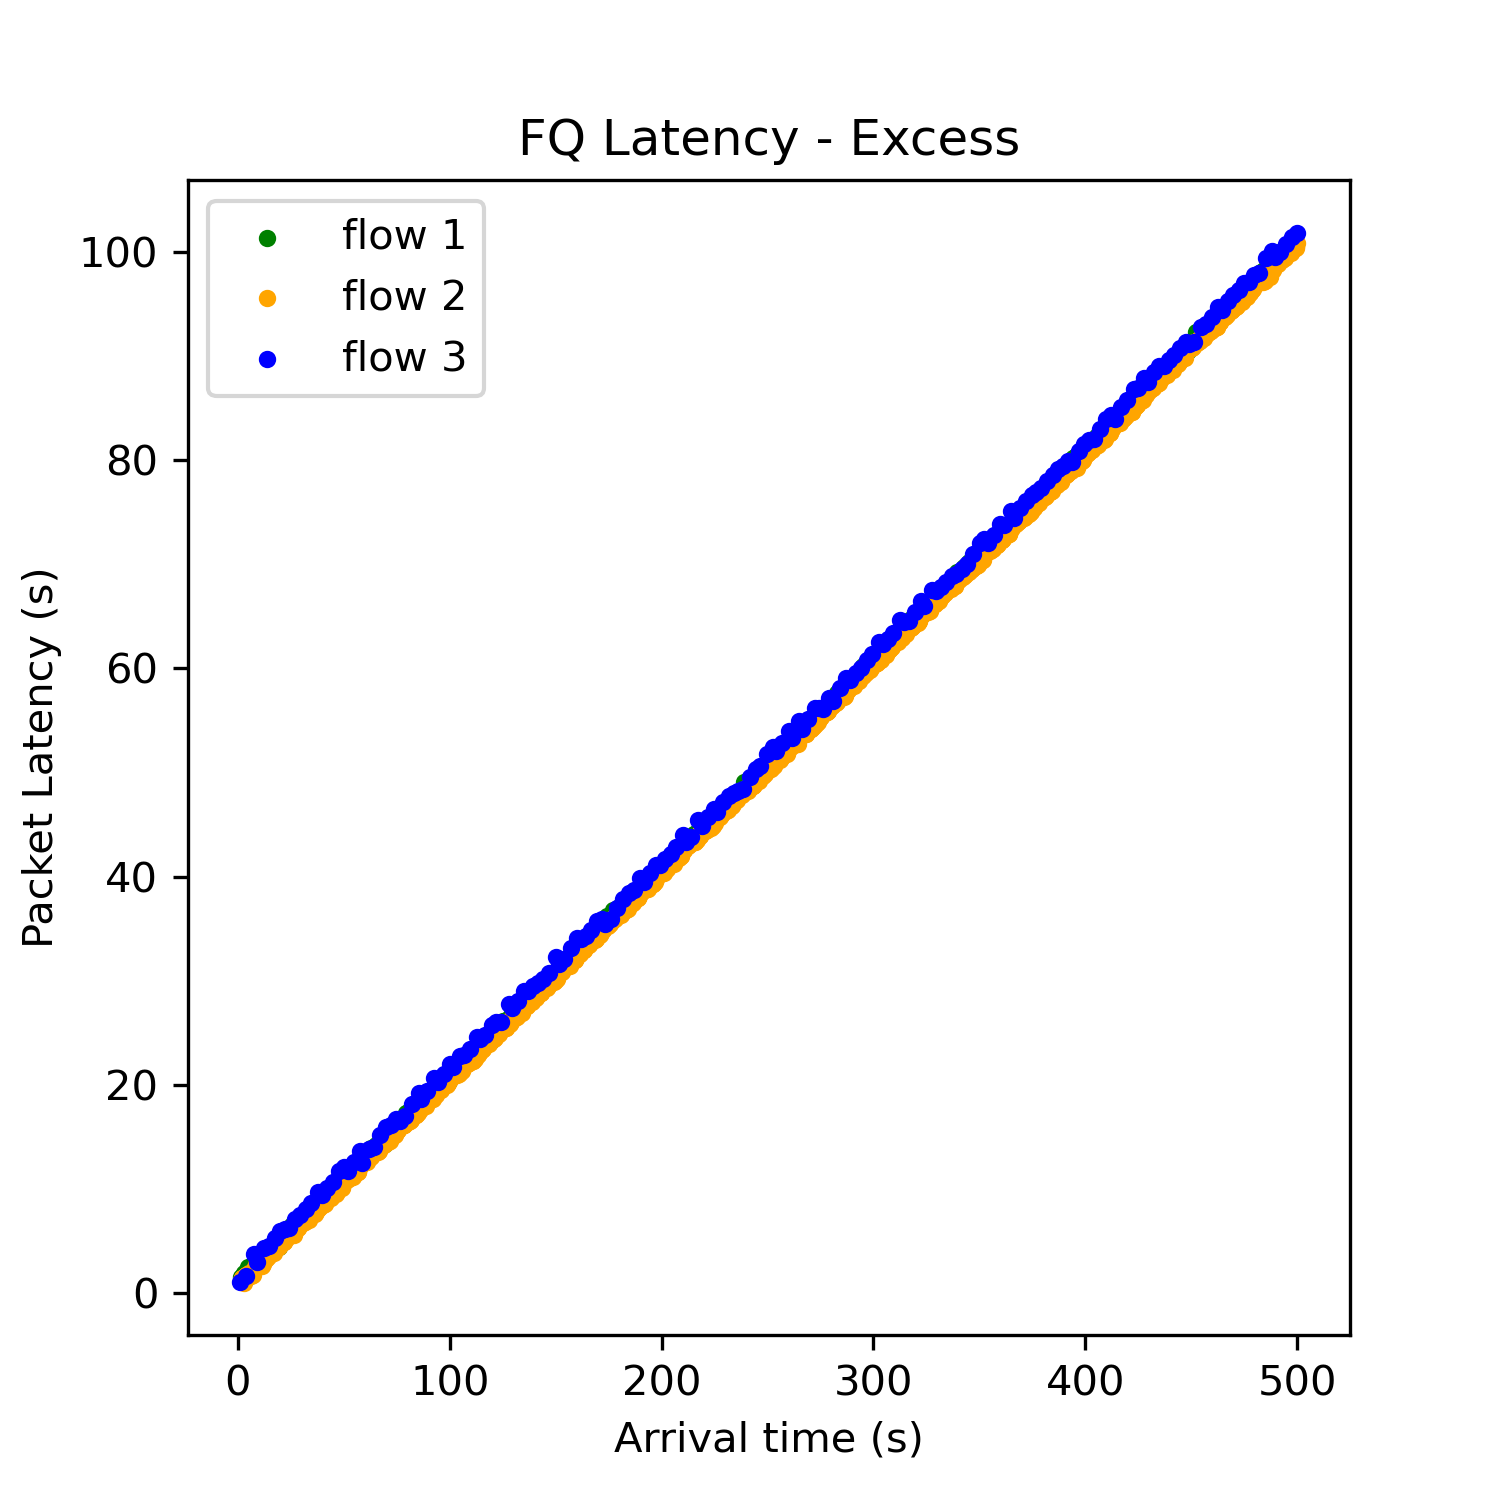
\includegraphics[width=\textwidth]{img/fq_excess}
                \end{figure}
            \end{column}
        \end{columns}
    \end{frame}


    \section{Conclusions}
    \subsection{Conclusions}
    \begin{frame}
        \frametitle{Conclusions}
        \begin{itemize}
            \item \alert{Interesting Result:} A single queue has the same result as a fair queue (for this test case)
            \item Round robin is a terribly unfair strategy for variable packets
            \begin{itemize}
                \item Even when the queues are moving
            \end{itemize}
            \item Modifying existing network simulation tools is dense work
            \begin{itemize}
                \item Would be great to have better documentation/compilation (thinking about NS-3)
            \end{itemize}
        \end{itemize}
    \end{frame}


    \section{Learning}

    \subsection{Learning}
    \begin{frame}
        \frametitle{Key Takeaways}
        \begin{enumerate}
            \item More advanced strategies aren't always better: sometimes a single queue can do the same work.
            \item Real time networks face a lot of challenges; unlike OS, networks are inherently less predictable.
            \item Real time networks have properties which aren't as easy to manipulate in existing simulators, like NS-3
        \end{enumerate}
    \end{frame}


\end{document}